\chapter{Conception}

\section*{Introduction}%
\addcontentsline{toc}{section}{\numberline{}Introduction}%
Ce chapitre est dédié à la conception de notre système de business intelligence. Nous allons commencer par présenter entièrement l’architecture du système à concevoir, puis nous allons concevoir chaqu’une des parties qui constituent le système. On débutera par le datawarehouse, duquel découlera les datamarts. Ensuite on passera à la conception des ETL qui seront charges d’alimenter notre datawarehouse. Passe cette étape on entamera avec la conception des cubes OLAP, dépendant des datamarts que nous avons construit pour faire nos analyses et nous finiront par concevoir nos tableaux de bords utilisables par le client. 

\section{Architecture du système de Business Intelligence}
Dans la phase d’analyse nous avons opté pour une plateforme de business intelligence. Ceci implique la conception du système des le début avec l’intégration des données jusqu’à la visualisation. 
\paragraph{}
Sur le plan technique et purement technique, la Business intelligence peut être caractérisée comme une famille d'outils progiciels bien spécifiques, chacun étant destiné à traiter une phase du processus décisionnel depuis la collecte de données au sein même des unités de production jusqu'à la facilitation de l'aide à la décision pour les managers. Voyons les caractéristiques typiques d'une plate-forme informatique décisionnelle, l'architecture du principe est ici classiquement présentée selon 4 étages.
\paragraph{}
La Business Intelligence (informatique décisionnelle) propose d'utiliser les données transitant par le Système d'information, données de production le plus souvent, en informations susceptibles d'être exploitées à des fins décisionnelles.

\begin{figure}[H]
    \centering
    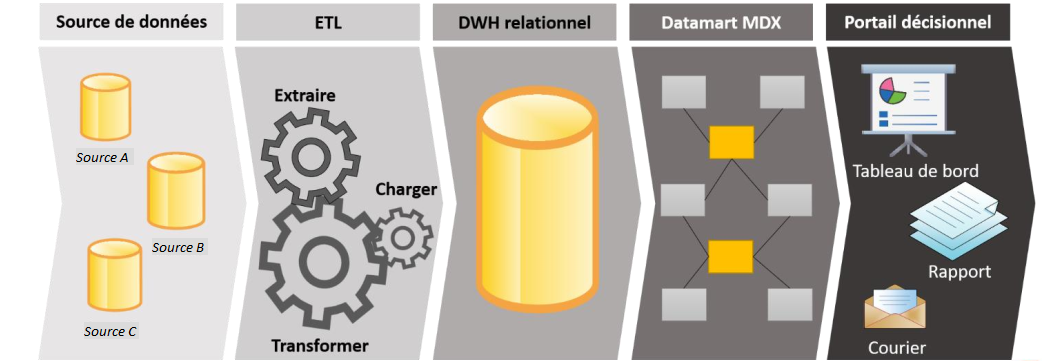
\includegraphics[width=\textwidth]{architecturesysteme}
    \caption{Architecture de notre Solution de Business Intelligence}
    \label{fig:architecturesysteme}
\end{figure}

La figure \ref{fig:architecturesysteme} montre l’architecture globale de notre système de business intelligence. On peut voir les 4 étages comme la transition entre les différents parties dans l'architecture.

\begin{itemize}
    \item \textbf{Collecter, nettoyer et consolider les données :} Extraire les données des systèmes de production et les adapter à un usage décisionnel. L'étage entre les sources de données et les processus ETL.
    \item \textbf{Stocker :} Centraliser les données structurées et traitées afin qu'elles soient disponibles pour un usage décisionnel. L'étage entre les processus ETL et le datawarehouse.
    \item \textbf{Distribuer :} Ou plutôt faciliter l'accessibilité des informations selon les fonctions et les types d'utilisation. L'étage entre le datawarehouse et les datamarts pour l'analyse.
    \item \textbf{Exploiter :} Ou comment assister du mieux possible l'utilisateur afin qu'il puisse extraire la substance de l'information des données stockées à cet usage. L'étage entre les datamarts et le portail décisionnel (les tableaux de bords).
\end{itemize}

\section{Conception du Datawarehouse et des Datamarts}
Les datawarehouse sont destinés à la mise en place de systèmes décisionnels. Ces systèmes, devant répondre à des objectifs différents des systèmes transactionnels, ont fait ressortir très vite la nécessité de recourir à un modèle de données simplifié et aisément compréhensible. La modélisation dimensionnelle permet cela. Elle consiste à considérer un sujet d’analyse comme un cube à plusieurs dimensions, offrant des vues en tranches ou des analyses selon différents axes.
\paragraph{}
La modélisation des bases de données relationnelles utilise les concepts d’entités et de relations afin de construire des tables. En business intelligence, la modélisation d’un datawarehouse (entrepôt de données) utilise les notions de table de faits et table de dimension. La figure \ref{fig:bddetdwh} extrait de la publication de Rachid SAAD\footnote{https://www.saadrachid.net/bi-big-data/modelisation-dun-datawarehouse/} sur la \textit{"MODÉLISATION D’UN DATAWAREHOUSE"} montre les différences entre la modélisation des bases de données et la modélisation d’un datawarehouse.

\begin{figure}[H]
    \centering
    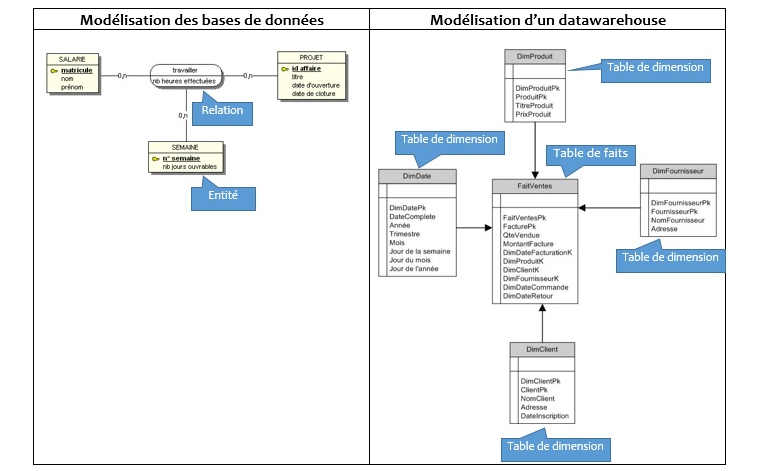
\includegraphics[width=\textwidth]{bddetdwh}
    \caption{Architecture basique de notre datawarehouse}
    \label{fig:bddetdwh}
\end{figure}

Mais d'abord parlons de l'architecture qu'aura le datawarehouse que nous voulons construire.

\subsection{Architecture du Datawarehouse}
Dans une architecture traditionnelle, il existe trois modèles communs de Data Warehouses : Data Warehouse virtuel, Data Mart et Data Warehouse d’entreprise :
\begin{itemize}
    \item \textbf{Un Data Warehouse virtuel :} C'est un ensemble de bases de données séparées, qui peuvent être interrogées ensemble, de sorte qu’un utilisateur peut accéder efficacement à toutes les données comme si elles étaient stockées dans un seul entrepôt de données.
    \item \textbf{Un modèle de Data Mart :}  C'est utilisé pour les rapports et les analyses spécifiques à un secteur d’activité. Dans ce modèle d’entrepôt de données, les données sont agrégées à partir d’une gamme de systèmes sources pertinents pour un domaine d’activité spécifique, comme les ventes ou la finance.
    \item \textbf{Un Data Warehouse d’entreprise :} Ceci implique que l’entrepôt de données doit contenir des données agrégées couvrant l’ensemble de l’organisation. Ce modèle considère l’entrepôt de données comme le cœur du système d’information de l’entreprise, avec des données intégrées provenant de toutes les unités d’affaires.
\end{itemize}

La structure du Data Warehouse d’une organisation dépend de sa situation actuelle et de ses besoins. La structure de base permet aux utilisateurs finaux de l’entrepôt d’accéder directement aux données sommaires dérivées des systèmes sources et d’effectuer l’analyse, la production de rapports et l’exploration de ces données. 

Nous allons implémenter un datawarehouse d'entreprise puisqu'elle répond le mieux a nos objectifs. La figure \ref{fig:architecturedwh} extrait du blog de Cartelis\footnote{https://www.cartelis.com/blog/architecture-data-warehouse}, représente bien l'architecture de notre datawarehouse.
\begin{figure}[H]
    \centering
    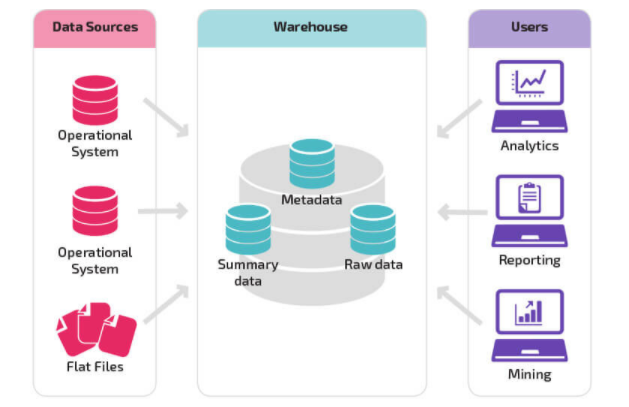
\includegraphics[width=\textwidth]{architecturedwh}
    \caption{Architecture basique de notre datawarehouse}
    \label{fig:architecturedwh}
\end{figure}

Cependent une zone staging est souvent nécessaire dans l'implémentation d'un datawarehouse. Comme mentionné plus haut, c'est la zone de préparation du datawarehouse. Dans la zone de préparation « Staging area » les données sont extraites à partir des sources de données, transformées et préparées pour le chargement final. Au niveau du serveur « ETL » il est procédé à l’affectation de clés artificielles et à quelques transformations nécessaires avant le chargement final dans la zone d’entreposage. Notre datawarehouse final aura une architecture comme dans la figure \ref{fig:architecturedwhfinal} extrait du même blog.

\begin{figure}[H]
    \centering
    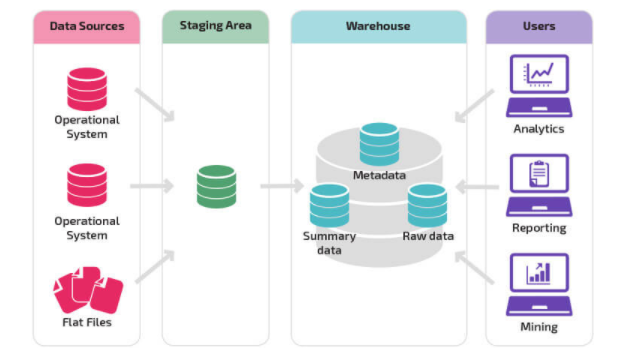
\includegraphics[width=\textwidth]{architecturedwhfinal}
    \caption{Architecture final de notre datawarehouse}
    \label{fig:architecturedwhfinal}
\end{figure}

\subsection{Modélisation dimensionnelle}
Dans un Data Warehouse (et au niveau de chaque Data mart), les données et leurs relations sont organisées suivant un modèle de données spécifique. Le diagramme \ref{fig:modeledimensionnel} qui représente un modèle dimensionnel ressemble à une étoile, avec une grande table centrale et un jeu de petites tables auxiliaires disposées en étoile autour de la table centrale. Celle-ci est appelée \textbf{table de faits} et les autres tables sont appelées \textbf{tables de dimensions}.

\begin{figure}[H]
    \centering
    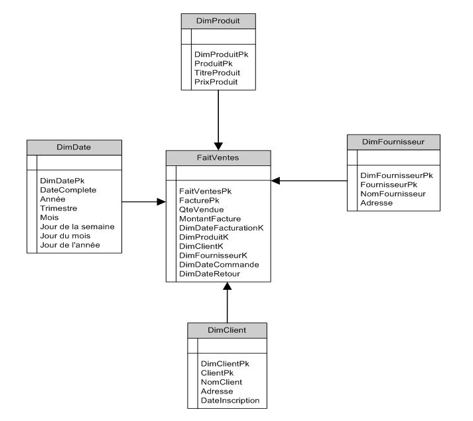
\includegraphics[width=\textwidth]{modeledimensionnel}
    \caption{Exemple de modèle dimensionnel de données}
    \label{fig:modeledimensionnelle}
\end{figure}

\subsubsection{Qu’est-ce qu’une table de fait?}
Une table de faits est la table centrale du modèle dimensionnel. Elle contient les informations observables (les mesures) sur ce qu’on veut analyser : Table de faits des ventes par exemple. Une ligne d’une table de faits correspond à une mesure. Ces mesures sont généralement des valeurs numériques, additives ; cependant des mesures textuelles peuvent exister mais sont rares. Une table de faits assure les liens plusieurs à plusieurs entre les dimensions. Elles comportent des clés étrangères, qui ne sont autres que les clés primaires des tables de dimension. Un peu comme dans les figures \ref{fig:structuretabledesfaits} et \ref{fig:exempletabledesfaits}

\begin{figure}[H]
    \centering
    \begin{minipage}{.6\textwidth}
      \centering
      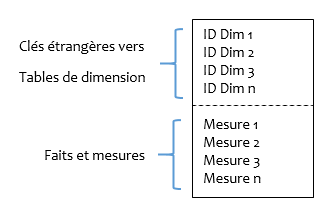
\includegraphics[width=.8\linewidth]{structuretabledesfaits}
      \captionof{figure}{Structure d'une table de faits}
      \label{fig:structuretabledesfaits}
    \end{minipage}%
    \begin{minipage}{.4\textwidth}
      \centering
      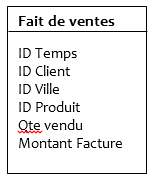
\includegraphics[width=.7\linewidth]{exempletabledesfaits}
      \captionof{figure}{Exemple d'une table de faits}
      \label{fig:exempletabledesfaits}
    \end{minipage}
\end{figure}

\subsubsection{Qu’est-ce qu’une table de dimension?}
Une table de dimension représente un axe d’analyse : dimension de temps, dimension géographique, dimension client, etc. Les tables de dimension sont les tables qui raccompagnent une table de faits, elles contiennent les descriptions textuelles de l’activité. Une table de dimension est constituée de nombreuses colonnes qui décrivent une ligne. C’est grâce à cette table que l’entrepôt de données est compréhensible et utilisable ; elles permettent des analyses en tranches et en dés. Une dimension est généralement constituée : d’une clé artificielle, une clé naturelle et des attributs. La figure \ref{fig:exempletablesdedimensions} illustre un exemple.

\begin{figure}[H]
    \centering
    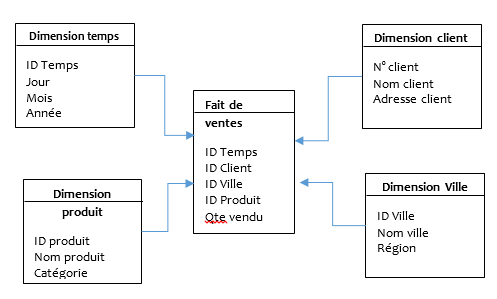
\includegraphics[width=\textwidth]{exempletablesdedimensions}
    \caption{Exemple de tables de dimension}
    \label{fig:exempletablesdedimensions}
\end{figure}

\subsection{Choix du modèle de schéma}
Trois modèles permettent la présentation d’un datawarehouse :
\begin{itemize}
    \item Modèle en étoile ;
    \item Modèle en flocon ;
    \item Modèle en constellation.
\end{itemize}

\subsubsection{Modèle en étoile}
Ce modèle se présente comme une étoile dont le centre n’est autre que la table des faits et les branches sont les tables de dimension. La force de ce type de modélisation est sa lisibilité et sa performance. La figure \ref{fig:exempletablesdedimensions} est un modèle en étoile.

\subsubsection{Modèle en flocon}
Identique au modèle en étoile, sauf que ses branches sont éclatées en hiérarchies. Cette modélisation est généralement justifiée par l’économie d’espace de stockage, cependant elle peut s’avérer moins compréhensible pour l’utilisateur final, et très couteuse en terme de performances. Un exemple dans la figure \ref{fig:exempleflocon}.
\begin{figure}[H]
    \centering
    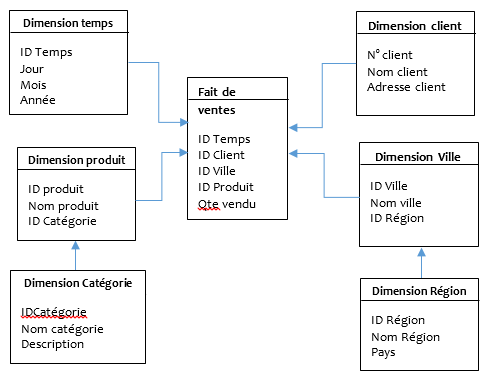
\includegraphics[width=\textwidth]{exempleflocon}
    \caption{Exemple de modèle en flocon}
    \label{fig:exempleflocon}
\end{figure}

\subsubsection{Modèle en constellation}
Ce n’est rien d’autre que plusieurs modèles en étoile liés entre eux par des dimensions communes. Comme dans la figure \ref{fig:exempleconstellation}
\begin{figure}[H]
    \centering
    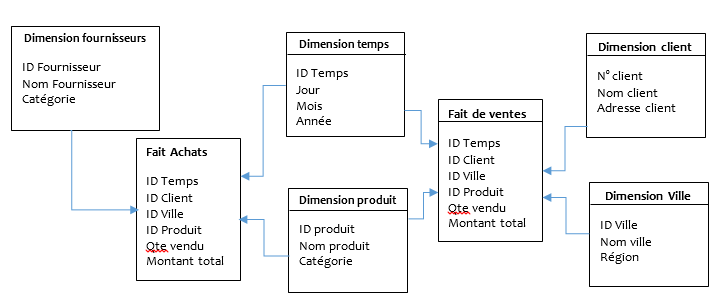
\includegraphics[width=\textwidth]{exempleconstellation}
    \caption{Exemple de modèle en constellation}
    \label{fig:exempleconstellation}
\end{figure}

Pour des raisons de performances nous avons choisi de travailler avec le \textbf{modèle en étoile}. Avec l'évolution de la technologie, l'espace mémoire n'est plus un grand soucis vu que nous travaillons principalement avec des données textuelles et numériques.

Ceci pourrait rapidement aboutir à un \textbf{modèle en constellation} si nous avons plus d'une table de fait par la suite.

\subsection{Méthode de construction}
\blindtext

\subsection{Construction des tables de faits et de dimensions}
\blindtext

\subsection{Conception du schéma global du Datawarehouse}
\blindtext

\subsection{Construction des Datamarts}
\blindtext 

\section{Conception des ETL}
\blindtext

\subsection{Architecture d’un processus ETL}
\blindtext

\subsection{Taches et étapes de l’ETL}
\blindtext

\subsection{Extraction des données}
\blindtext

\subsection{Transformation des données}
\blindtext

\subsection{Chargement des données}
\blindtext

\subsection{Schémas des ETL conçus }
\blindtext

\section{Conception des cubes OLAP}
\blindtext

\section{Conception du reporting (La visualisation) - La méthode UI/UX}
\blindtext

\section*{Conclusion}%
\addcontentsline{toc}{section}{\numberline{}Conclusion}%
\blindtext

